\documentclass[12pt,letterpaper]{article}
\usepackage[papersize={8.5in,11in}]{geometry}
\usepackage{fullpage}
\usepackage{gensymb}
\usepackage[utf8]{inputenc}
\usepackage{graphicx}
\usepackage{amsmath,amsfonts,mathtools,amsthm}
\author{Jiaqi Zhu \\Amath 482, Winter 2020}
\title{An Ultrasound Problem}

\begin{document}
\maketitle
\begin{abstract}
Ultrasound is used to locate the postion of the marble in a dog's intestine; however, the data obtained is highly noisy. In order to locate the exact marble's position, we apply the Fast Fourier Transform to analyze the twenty data measurments in the frequency domain. After determining the center frequency through averaging of the spectrums, we filiter the data around the center freqeuncy to be less noisy and determine the path of the marble. Finally, the final position of the marble is detected and we could destroy the marble to save the dog's life. 
\end{abstract}

\section*{I. Introduction and Overview}
A dog accidentally swallowed a marble which has now worked its way into the intestines. Ultrasound is used to locate the marble's position; however, the dog keeps moving and the internal fluid movement through the intestines generates highly noisy data. There are 20 rows
of data for 20 different measurements that were taken in time. In order to save the dog's life, we must locate and compute the trajectory of the marble. 
\\
\\We can solve this problem in the following three steps:
\\1. Determine the center frequency through the averaging of 20 spectrums. 
\\2. Filter the data to denoise and determine the path
\\3. Determe the final position of the marble, namely,the position of the 20th data measurment.
\\
\\After locating the exact position of the marble, we could apply an intense acoustic wave to breakup the marble so that the dog is saved.  
\section*{II. Theoretical Background}
\subsection*{Fourier Transform}
The Fourier transform is an integral transform of time or signal into its frequencies. The inverse Fourier transform is just an integral transform of the frequency back to the time or the signal. The Fourier transform and its inverse are defined as:
$$\mathcal{F}(k) = \dfrac{1}{\sqrt{2\pi}}\int_{-\infty}^{\infty}e^{-ikx}f(x)dx$$
$$f(k) = \dfrac{1}{\sqrt{2\pi}}\int_{-\infty}^{\infty}e^{ikx}\mathcal{F}(x)dx$$
Formally, the transform is over the entire real line $x\in [-\infty, \infty]$; however, in the application, our domain is finite, which is $x \in [-L,L]$. Moreover, $e^{\pm{ikx}} = \cos(kx)\pm{i\sin(kx)}$ describes the oscillary behavior. 
\subsection*{Fast Fourier Transform (FFT)}
The Fast Fourier Transform is an algorithm to perform the forward and backward Fourier transforms.It finds the transform on an interval $x \in [-L,L]$ because the integration Kernal $\exp(ikx)$ is oscillary and thus the solution in this interval is periodic. FFT is very powerful because the operation count for solving a system could drop to $O(N\log(N))$ by discretizing the range  $x \in [-L,L]$  into $2^n$ points. Aside from transforming the function, it does three major things:
\\1. shift the data from one side to the other about 0. 
\\2. mutiplies every other mode by -1.
\\3. assumes we are working on a $2\pi$ periodic domain. 

\subsection*{FFT Application: Filtering and Averaging}
\subsubsection*{Filtering}
FFT have be applied in the field of digital signal processing and imaging because it can be used to analyze the data in the frequency domain. In most applications, the signals are not very ideal and will always have lots of noise to break our analysis. In order to improve the ability to detect the signal with the noise, which means to denoise the data, we firstly apply a FFT to transform the signal to the frequency domain. Then we could apply the Gaussian Filter to determine the signal center frequency. The Gaussian Filter is defined as following:
$$\mathcal{F}(k) = \exp(-\tau(k-k_0)^2)$$
where $\tau = 0.2$, which measures the bandwidths of the filter, k is the wavenumber and $k_0$ is the center frequency. The filter tends to isolate the signal input around $k_0$ in order to attenuate the noise. 
\\After applying the Gaussian Filter, we can invert the Fourier Transform to repoduce an approximation to the signal field. 
\subsubsection*{Averaging}
However, we may not always know the center frequency $k_0$, then gaussian filter isn't enough for us to attenuate the noise. The white noise and more signal data derived from gaussian filter could provide more information for us. Consider that the white noise can be modeled adding a normally distributed random variable with zero mean to each Fourier component of the spectrum. It means that when we add up all the white noise, on average, it should be zero. Then it could be easy for us to accurately detect a signal. 

\section*{III. Algorithm Implementation and Development}
For this utrasound problem, there are 20 rows of data for 20 different measurements that were taken in time, each of which contains the signal data of the position of the marble but is noisy because of the internal fluid movement in the dog's intestines. In order to determine the final position of the marble in order to save the dog's life, I apply FFT to analyze the data in its frequency domain. The problem could be solved in the three steps given in the introduction.
\subsection*{1. Determine the center frequency through the averaging of 20 spectrums. }
In order to determine the center frequency, firstly I sum up the FFT of the 20 measurements by for loop and divided by 20 to get the average. Then the noise should be attenuated because the mean of the noise, on average, should be zero. Suppose that the maximum frequency is generated by the marble, we could find the index of the maximum frequency and locate the center frequency. 
\subsection*{2. Filter the data to denoise and determine the path}
We will apply the gaussian filter to denoise the system. The Gaussian filter we used here is 
$$ \exp(-0.2*((Kx-kxc).^2+(Ky-kyc).^2+(Kz-kzc).^2))$$
to isolate the signal of the marble around kxc,kyc,kzc in order to attenuate the noise. Then for each measurement, we apply FFT to derive the freqeuncy and apply the Gaussian filter in order to denoise the system. Then we will inverse the Fourier transform (IFFT) to reproduce the signal field of the marble. Then we find the index of the maximum frequency and locate the position of the marble (xp,yp,zp) for each data measurement. 
\subsection*{3. Determe the final position of the marble, namely,the position of the 20th data measurment.}
Finally, we could just return the 20th measurement of (xp,yp,zp) to derive the exact final position of the marble. 

\section*{IV. Computational Results}
At first, we can see that the signal of marble is highly noisy. Here's the plot of the marble signal for the first data measurement:
\begin{center}
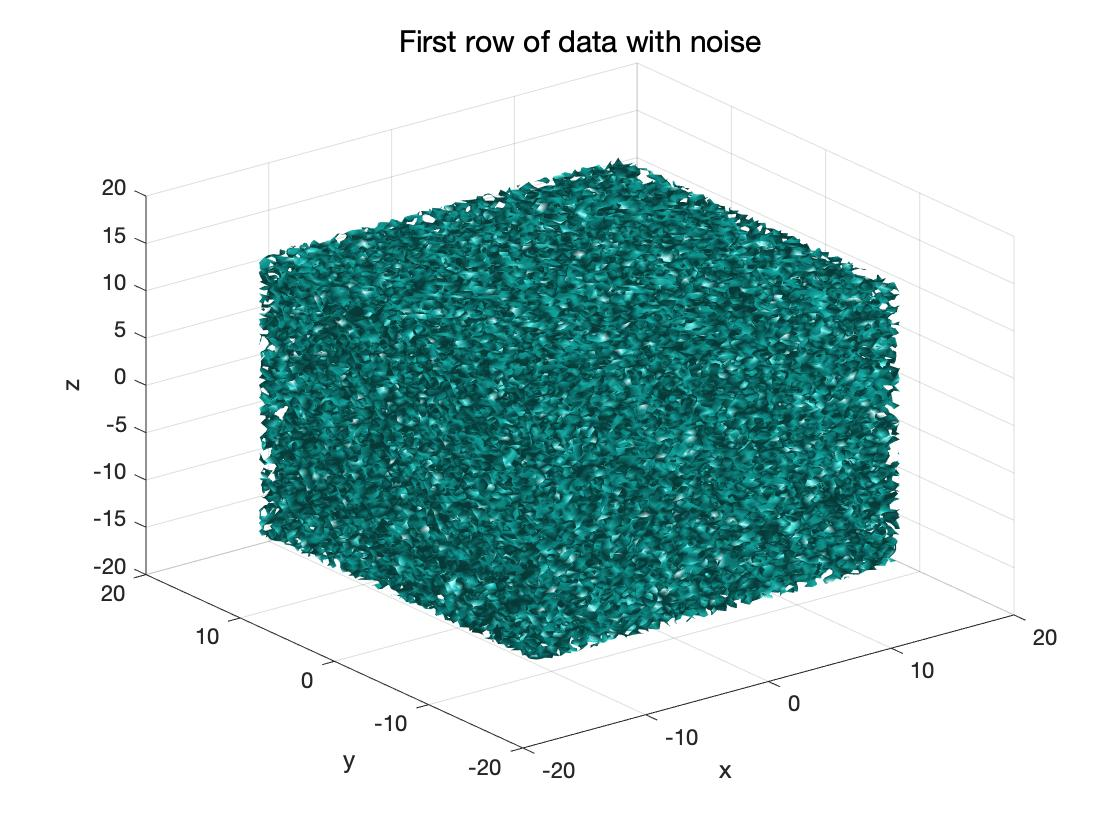
\includegraphics[height= 4 in]{1.jpg}
\end{center}
Through averaging the 20 spectrums, we obtain that the center frequency generated by the marble is at (1.8850,-1.0472,0). Based on the center frequency we obtained, we apply the Gaussian Filter to denoise the system and locate the marble for each data measurement
Finally, we derive the exact final position of the marble (-5.6250, 4.2188, -6.0938). Here's the plot of the path and the destination of the marble:
\begin{center}
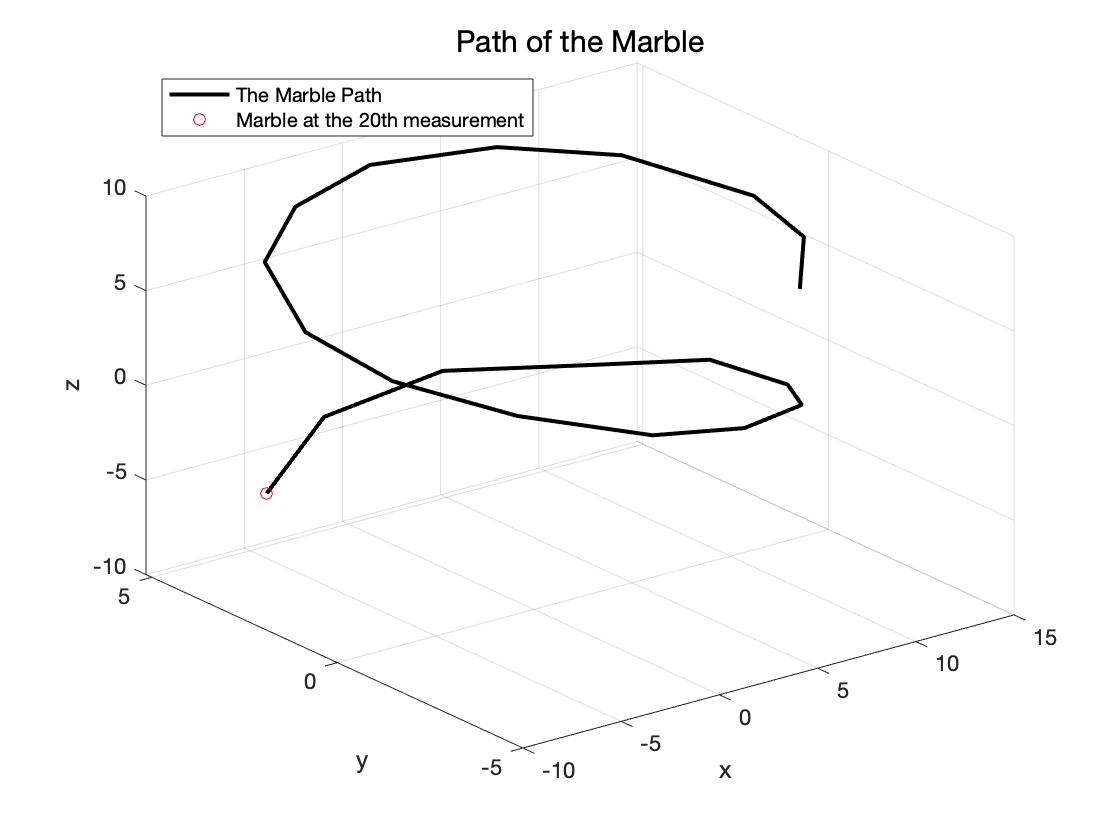
\includegraphics[height= 4 in]{2.jpg}
\end{center}
Luckily, the marble is detected and my dog could be alive!
\section*{V. Summary and Conclusions}
Ultrasound is used to locate the marble in the dog's intestines; however, the data we obtained is highly noisy because of the internal fuild movement in the dog's intestine. In order to denoise the system the determine the exact position of the marble, we apply FFT to manipulate the data in its frequency domain. Through averaging of the 20 spectrums, we could determine the center frequency. Given the center frequency generated by the marble, we apply the Gaussian Filter to attenuate the noise from the frequency and then locate the exact position of the marble in each measurement, thus determining the path of the marble. Consequently, we figure out the final destination of the marble and save the dog's life. From this problem, we could see the power of FFT through filtering and averaging to locate the position of an object even if the signals are highly noisy.
\newpage 
\section*{Appendix A. MATLAB functions used and brief implementation explanation}
meshgrid: [X,Y,Z]=meshgrid(x,y,z) returns 3-D grid coordinates defined by x, y, z. 
\\
\\reshape: Un(:,:,:)=reshape(Undata(j,:),n,n,n) changed Undata(j,:) to a n by n by n array.
\\
\\fftn: fftn(Un) performs N-D Fast Fourier Transform on Un.
\\
\\fftshift: fftshift(Uavg) shifts the transformed function back to its mathematically correct
positions.
\\
\\abs:  abs(fftshift(Uavg)) returns the absolute value of fftshift(Uavg). 
\\
\\max: max(Uavg(:)) returns the maxmium value in Uavg(:)
\\
\\ind2sub: [xi,yi,zi]=ind2sub(size(Uavg),index) returns 3 arrays xi, yi, zi containing the equivalent multidimensional subscripts corresponding to the linear indices index for Uavg. 
\\
\\ifftshift: ifftshift(Unft) rearranges a zero-frequency-shifted Fourier transform Unft back to the original transform output.
\\
\\ifftn: ifftn(ifftshift(Unft)) performs inverse N-D Fast Fourier Transform on ifftshift(Unft).
\\
\\isosurface: isosurface(X,Y,Z,abs(Un),0.4) computes isosurface data from the volume data abs(Un). 
\\
\\plot3: plot3(xp,yp,zp,'k','Linewidth',[2]) plots in 3D space. 
\newpage
\section*{Appendix B. MATLAB codes}
\begin{verbatim}
clear; close all; clc;
load Testdata
L=15; % spatial domain
n=64; % Fourier modes
x2=linspace(-L,L,n+1); x=x2(1:n); y=x; z=x;
k=(2*pi/(2*L))*[0:(n/2-1) -n/2:-1]; ks=fftshift(k);
[X,Y,Z]=meshgrid(x,y,z);
[Kx,Ky,Kz]=meshgrid(ks,ks,ks);

% first row data with noise
Un(:,:,:)=reshape(Undata(1,:),n,n,n);
isosurface(X,Y,Z,abs(Un),0.4)
axis([-20 20 -20 20 -20 20]), grid on, drawnow
title('First row of data with noise','Fontsize',[15])
xlabel('x'),ylabel('y'),zlabel('z');

% determine the center frequency through averaging of the spectrum
Uavg2 = zeros(1,n^3);
Uavg = reshape(Uavg2,n,n,n);
for j=1:20
Un(:,:,:)=reshape(Undata(j,:),n,n,n);
Uavg = Uavg+fftn(Un);
end
Uavg = abs(fftshift(Uavg))/20;
[value1, index] = max(Uavg(:));
[xi,yi,zi]=ind2sub(size(Uavg),index);
kxc=Kx(xi,yi,zi);
kyc=Ky(xi,yi,zi);
kzc=Kz(xi,yi,zi);

% filter the data to denoise and determine the path 
gaussianf = exp(-0.2*((Kx-kxc).^2+(Ky-kyc).^2+(Kz-kzc).^2));
for j = 1:20
Un(:,:,:)=reshape(Undata(j,:),n,n,n);
Unft = fftshift(fftn(Un)).*gaussianf;
Unf = ifftn(ifftshift(Unft));
[value2,index2] = max(Unf(:));
[xj,yj,zj]=ind2sub(size(Unf),index2);
xp(j)=X(xj,yj,zj);
yp(j)=Y(xj,yj,zj);
zp(j)=Z(xj,yj,zj);
%close all,isosurface(X,Y,Z,abs(Unf),0.4)
%axis([-20 20 -20 20 -20 20]),
%xlabel('x'),ylabel('y'),zlabel('z'),grid on
end
plot3(xp,yp,zp,'k','Linewidth',[2])
hold on
plot3(xp(20),yp(20),zp(20),'or')
legend({'The Marble Path','Marble at the 20th measurement'},'Location','northwest')
title('Path of the Marble', 'Fontsize', [15])
xlabel('x'),ylabel('y'),zlabel('z'),grid on
% Destination of the path
[xp(20),yp(20),zp(20)]
\end{verbatim}
\section*{Reference}
\begin{verbatim}
Kutz, Jose Nathan. Data-Driven Modeling & Scientific Computation: Methods 
	    for Complex Systems & Big Data. Oxford University Press, 2013.
\end{verbatim}
\end{document}